\section{Methodology and Evaluation}

We compare PPA metrics of Saturn VU+OPU against Saturn VU for different vector lengths, VLEN, the number of bits per vector register. We first study how performance scales with VLEN in the ideal case of a GEMM kernel, and then evaluate more realistic quantized DNN workloads. To do so, we use two complementary software paths. The first is a library-based path built from ExecuTorch, XNNPACK, and Zephyr, which exposes OPU kernels inside an embedded inference stack and is useful for bring-up, instrumentation, and kernel-level profiling. The second is a compiler-based path built on IREE, which applies graph and lowering transformations to rewrite larger portions of the model into OPU-supported forms and evaluates the resulting end-to-end speedup.

\subsection{PyTorch Integration}

\begin{figure*}[t]
  \centering
  \begin{minipage}[t]{0.52\textwidth}
    \centering
    \includegraphics[width=\linewidth]{figures/software_flow_opu.png}
  \end{minipage}\hfill
  \begin{minipage}[t]{0.43\textwidth}
    \centering
    \includegraphics[width=\linewidth]{figures/IREE-flow.png}
  \end{minipage}
  \caption{Two complementary software paths used in this work. Left: library-based deployment flow using ExecuTorch, XNNPACK, and Zephyr. Right: compiler-based IREE flow that rewrites model subgraphs into a small number of OPU-supported kernel families and deploys them through an adapted IREE runtime.}
  \label{fig:sw-flows}
\end{figure*}

To enable hardware-software co-design for the Saturn VU+OPU SoC, we build automated flows for compiling and evaluating PyTorch models. Figure~\ref{fig:sw-flows} contrasts the two software paths used in this work. The library-based path starts from ExecuTorch model export, partitions the graph to XNNPACK operators, and executes those operators on Zephyr using \texttt{pthreadpool} worker threads pinned across the multicore SoC. The compiler-based path starts from the same quantized model but uses IREE to canonicalize, pattern match, tile, and lower larger subgraphs into a small number of Saturn-specific kernel families before deployment.

The library path and the compiler path serve different purposes. The library path gives direct access to individual kernels inside a realistic embedded runtime, making it the most useful environment for bring-up, instrumentation, and profiling of OPU microkernels at fine granularity. The compiler path is instead aimed at end-to-end deployment: rather than hand-enabling one operator at a time, it increases model coverage by rewriting multiple layer families into forms that can share the same OPU lowering.

Supporting the library stack required modifications to the surrounding software environment. We extended Zephyr to support RVV lazy context switching, updated the toolchain to support RVV intrinsics, and added thread pinning support to the Zephyr POSIX interface so that XNNPACK's worker threads could be mapped cleanly onto cores. We also modified XNNPACK to build as a static library against Zephyr's POSIX implementation, enabling multicore bare-metal execution from ExecuTorch models rather than only single-threaded reference kernels.

\subsection{Outer Product Kernel Integration}\label{sec:xnnpack-kernel}

We first enabled Saturn OPU through XNNPACK microkernels. This library route was essential for understanding kernel behavior before moving to full end-to-end compilation. It allowed us to isolate the effects of tile shape, packing, activation layout, fused epilogues, and thread-dispatch overhead while keeping the rest of the runtime stack realistic.

Because GCC does not yet provide intrinsic support for the Saturn matrix instructions, we expose the OPU through assembly macros for matrix and vector registers and use them to implement \texttt{int8} GEMM kernels with fused activation. Compared to RVV microkernels, which are limited by VRF capacity and operate on tiles up to roughly \texttt{7x4$v_l$}, the OPU microkernels operate on larger \texttt{$v_l$x$v_l$} tiles. This reduces the number of dispatched microkernels per operator and lowers runtime overhead.

The main kernel-level challenge is data layout. Optimized RVV microkernels assume row-major activations, but the OPU kernel would then require strided vector loads, creating a bottleneck at the load-store unit. To avoid this, the OPU kernels repack activations into column-major order so that the inner loop can use unit-stride loads. In XNNPACK this repacking is done at runtime, which is appropriate for operator-level experimentation and profiling. These library-side experiments made clear that OPU performance depends not only on the inner instruction sequence, but also on packing, layout, and dispatch overhead. Those observations directly informed the compiler-side transformations described next.

\subsection{IREE-Based Bare-Metal Compilation}\label{sec:iree-compilation}

In addition to the ExecuTorch/XNNPACK software stack, we develop an IREE-based flow to study Saturn OPU lowering and runtime overheads in a modern compiler stack. This flow extends IREE with Saturn-specific lowering, including target-aware int8 tile selection, RISC-V ukernel support, and a direct-output encoding path for matrix multiplication. Rather than using IREE only as an IR generator, we use it as the full ahead-of-time compilation and invocation stack on FireSim, allowing us to measure both code generation quality and the fixed overheads that remain visible during deployment.

The key difference from the library path is scope. In XNNPACK, OPU support is introduced by writing and wiring up individual kernels. In IREE, the goal is instead to increase the fraction of model compute that can be rewritten into OPU-supported forms. Dense layers lower directly into OPU matmul. Transformer-style models first collapse multi-\(N\) contractions into standard 2D matmuls so that attention projections and related dense subgraphs can reuse the same lowering. CNN-style models convert convolutions into im2col-plus-matmul. We also add a fused quantized path that combines matmul with dequantization, requantization, and store into an OPU-aware ukernel. In this way, the compiler generalizes across layer families by reducing them to a small set of contraction-centric kernel patterns instead of requiring a separate hardware path for each high-level operator.

This compiler flow was guided by the same issues exposed in the library-level experiments: tile selection, packing overhead, layout materialization, and epilogue fusion. For a \(1024\times 1024\times 1024\) int8 GEMM on the Saturn OPU V128-D64 FireSim configuration, the optimization sequence improves performance from 0.84 ops/cycle in the initial path to 14.6 ops/cycle after correcting tile selection, 34.8 ops/cycle after unrolling the K-loop by four, 39.0 ops/cycle after hoisting constant-weight packing, and 57.9 ops/cycle in the final direct-output path. Throughput is reported as \(2MNK\) divided by measured cycles around the full invocation, so the reported values include VM and HAL overheads, packing, fill operations, and the final ukernel dispatch in addition to OPU compute. Relative to the 128 ops/cycle peak of the V128-D64 configuration, the final \(1024^3\) point reaches 45.3\% utilization. Across square int8 GEMMs from \(64^3\) to \(2048^3\), the optimized OPU path improves from 3.95 to 65.62 ops/cycle, corresponding to 3.1\%--51.3\% utilization of peak and a 2.4\(\times\)--52.5\(\times\) speedup over the RVV baseline. These results show that, for the tightly-coupled OPU, compiler control of tiling, packing, and layout materialization is as important as the inner-kernel implementation itself.

\begin{figure*}[t]
  \centering
  \begin{minipage}[t]{0.48\textwidth}
    \centering
    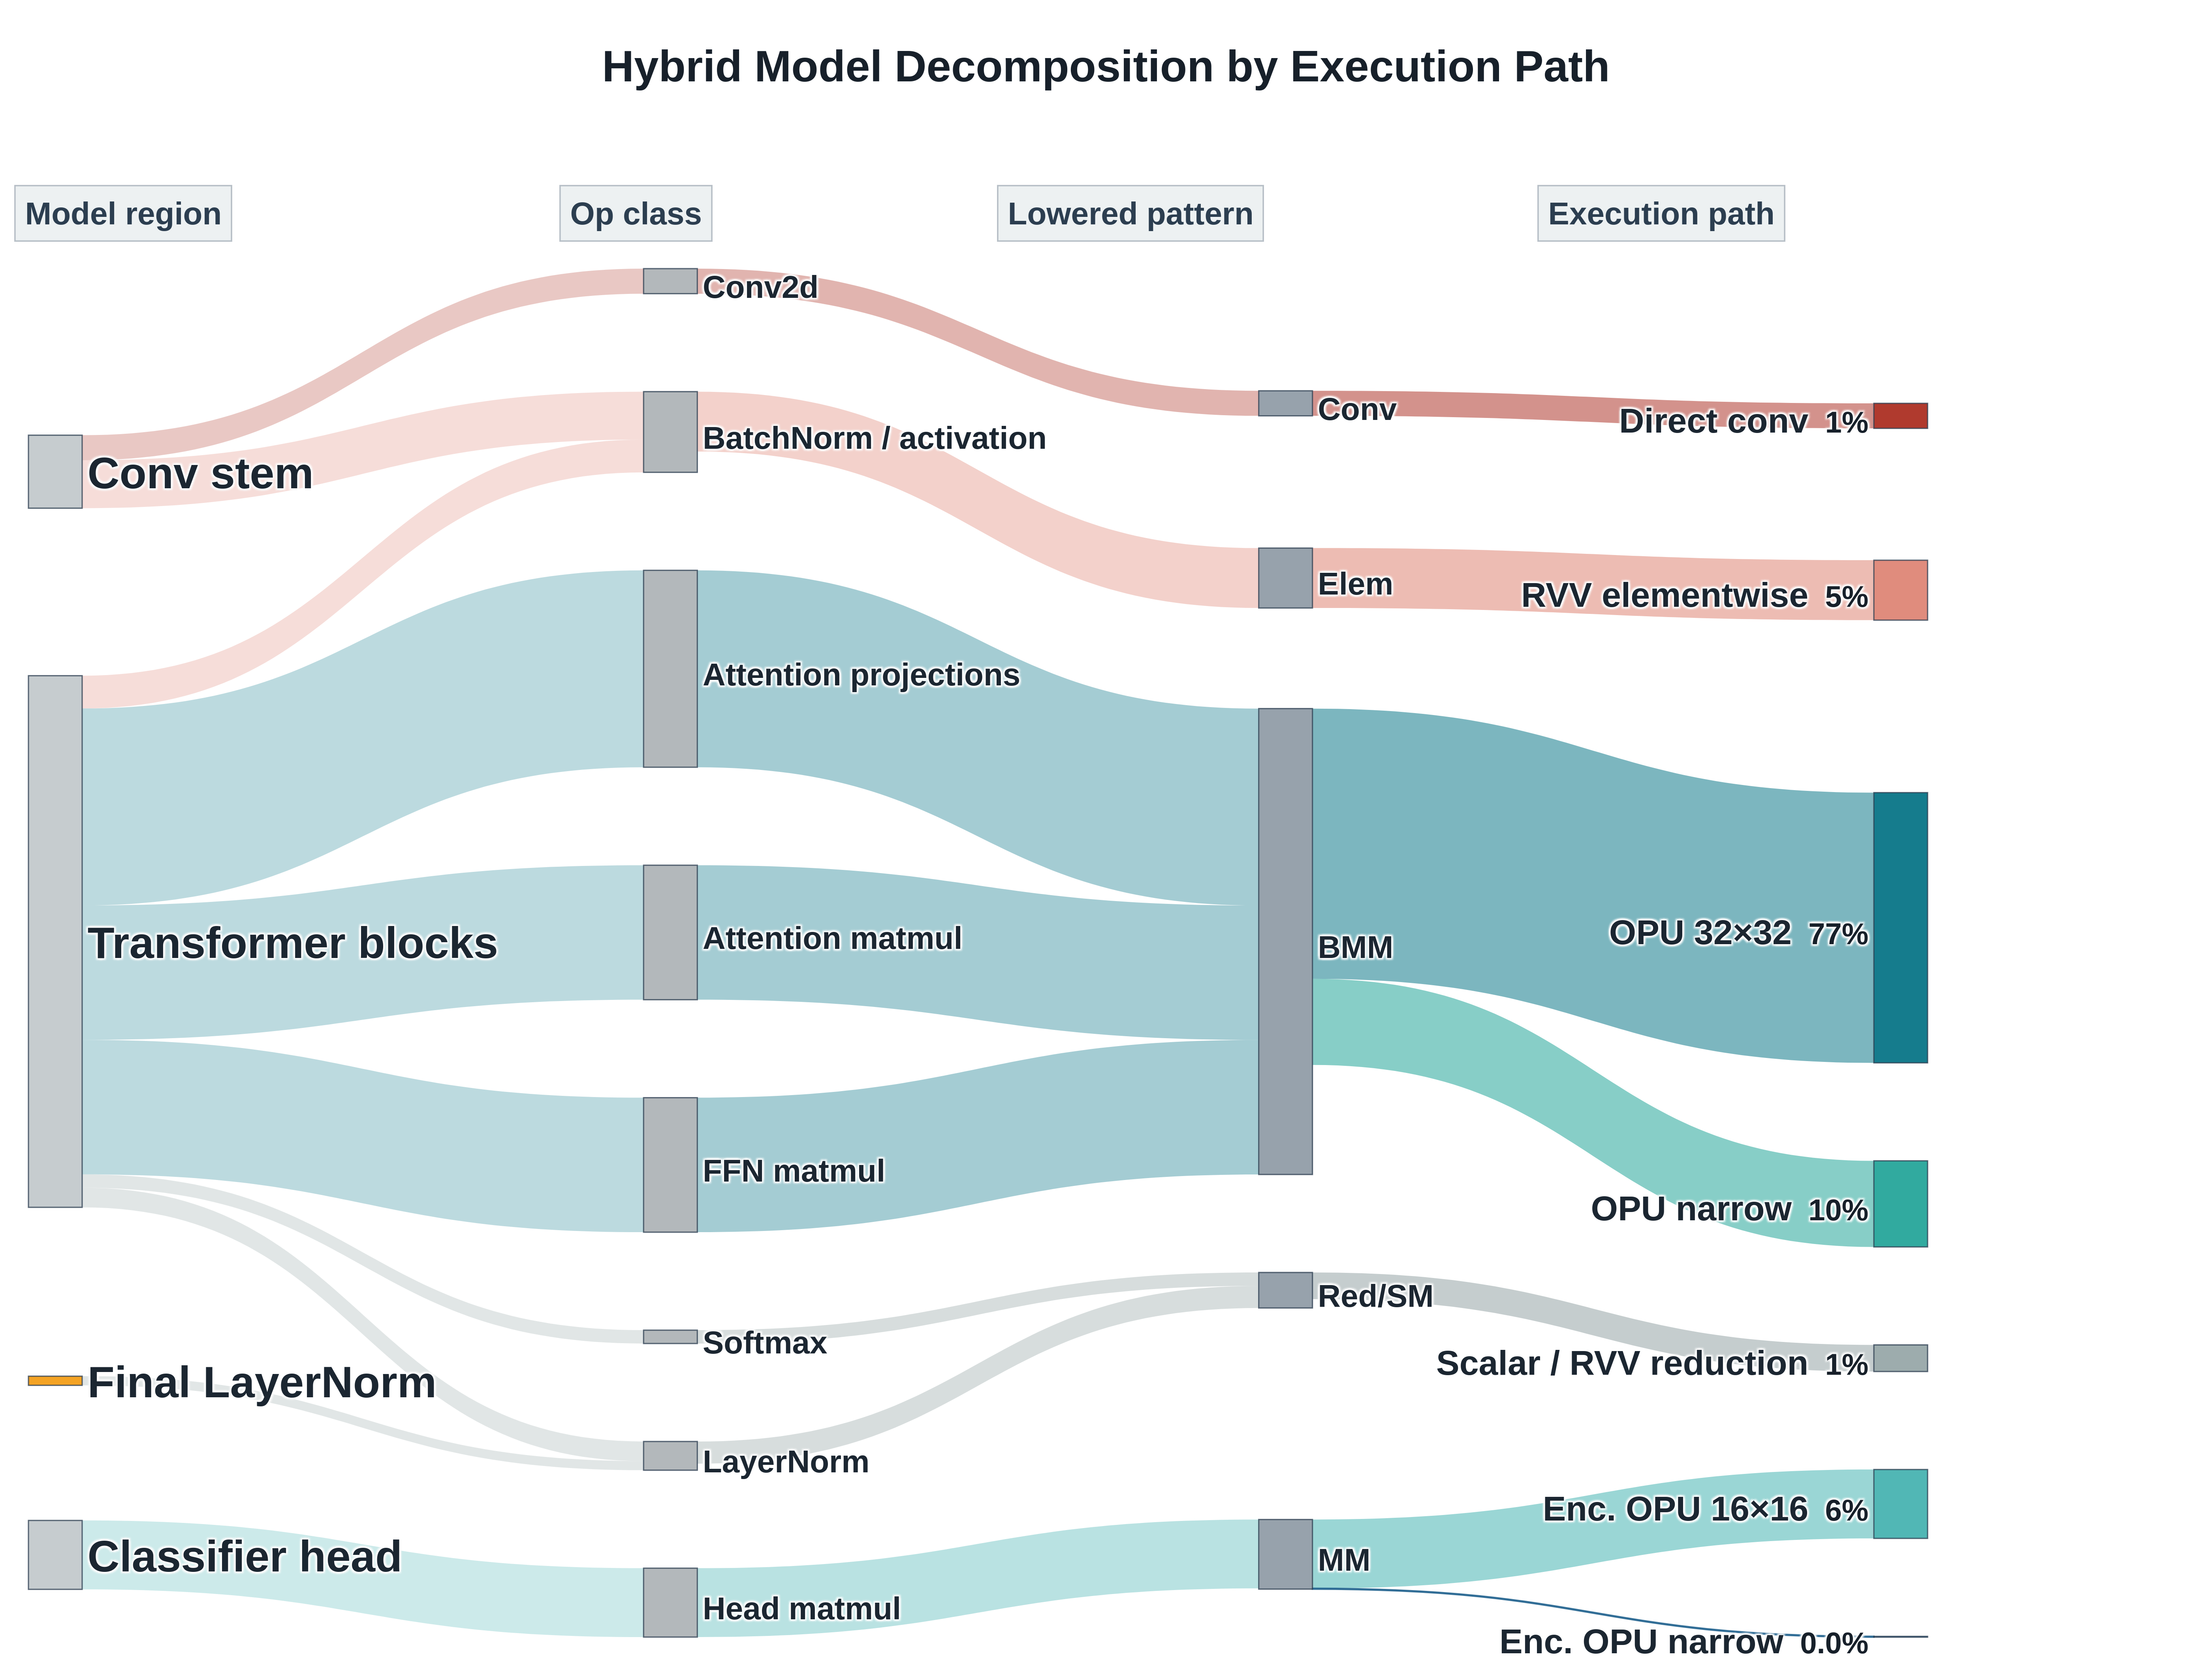
\includegraphics[width=\linewidth]{figures/sankey_hybrid_paper.png}
  \end{minipage}\hfill
  \begin{minipage}[t]{0.48\textwidth}
    \centering
    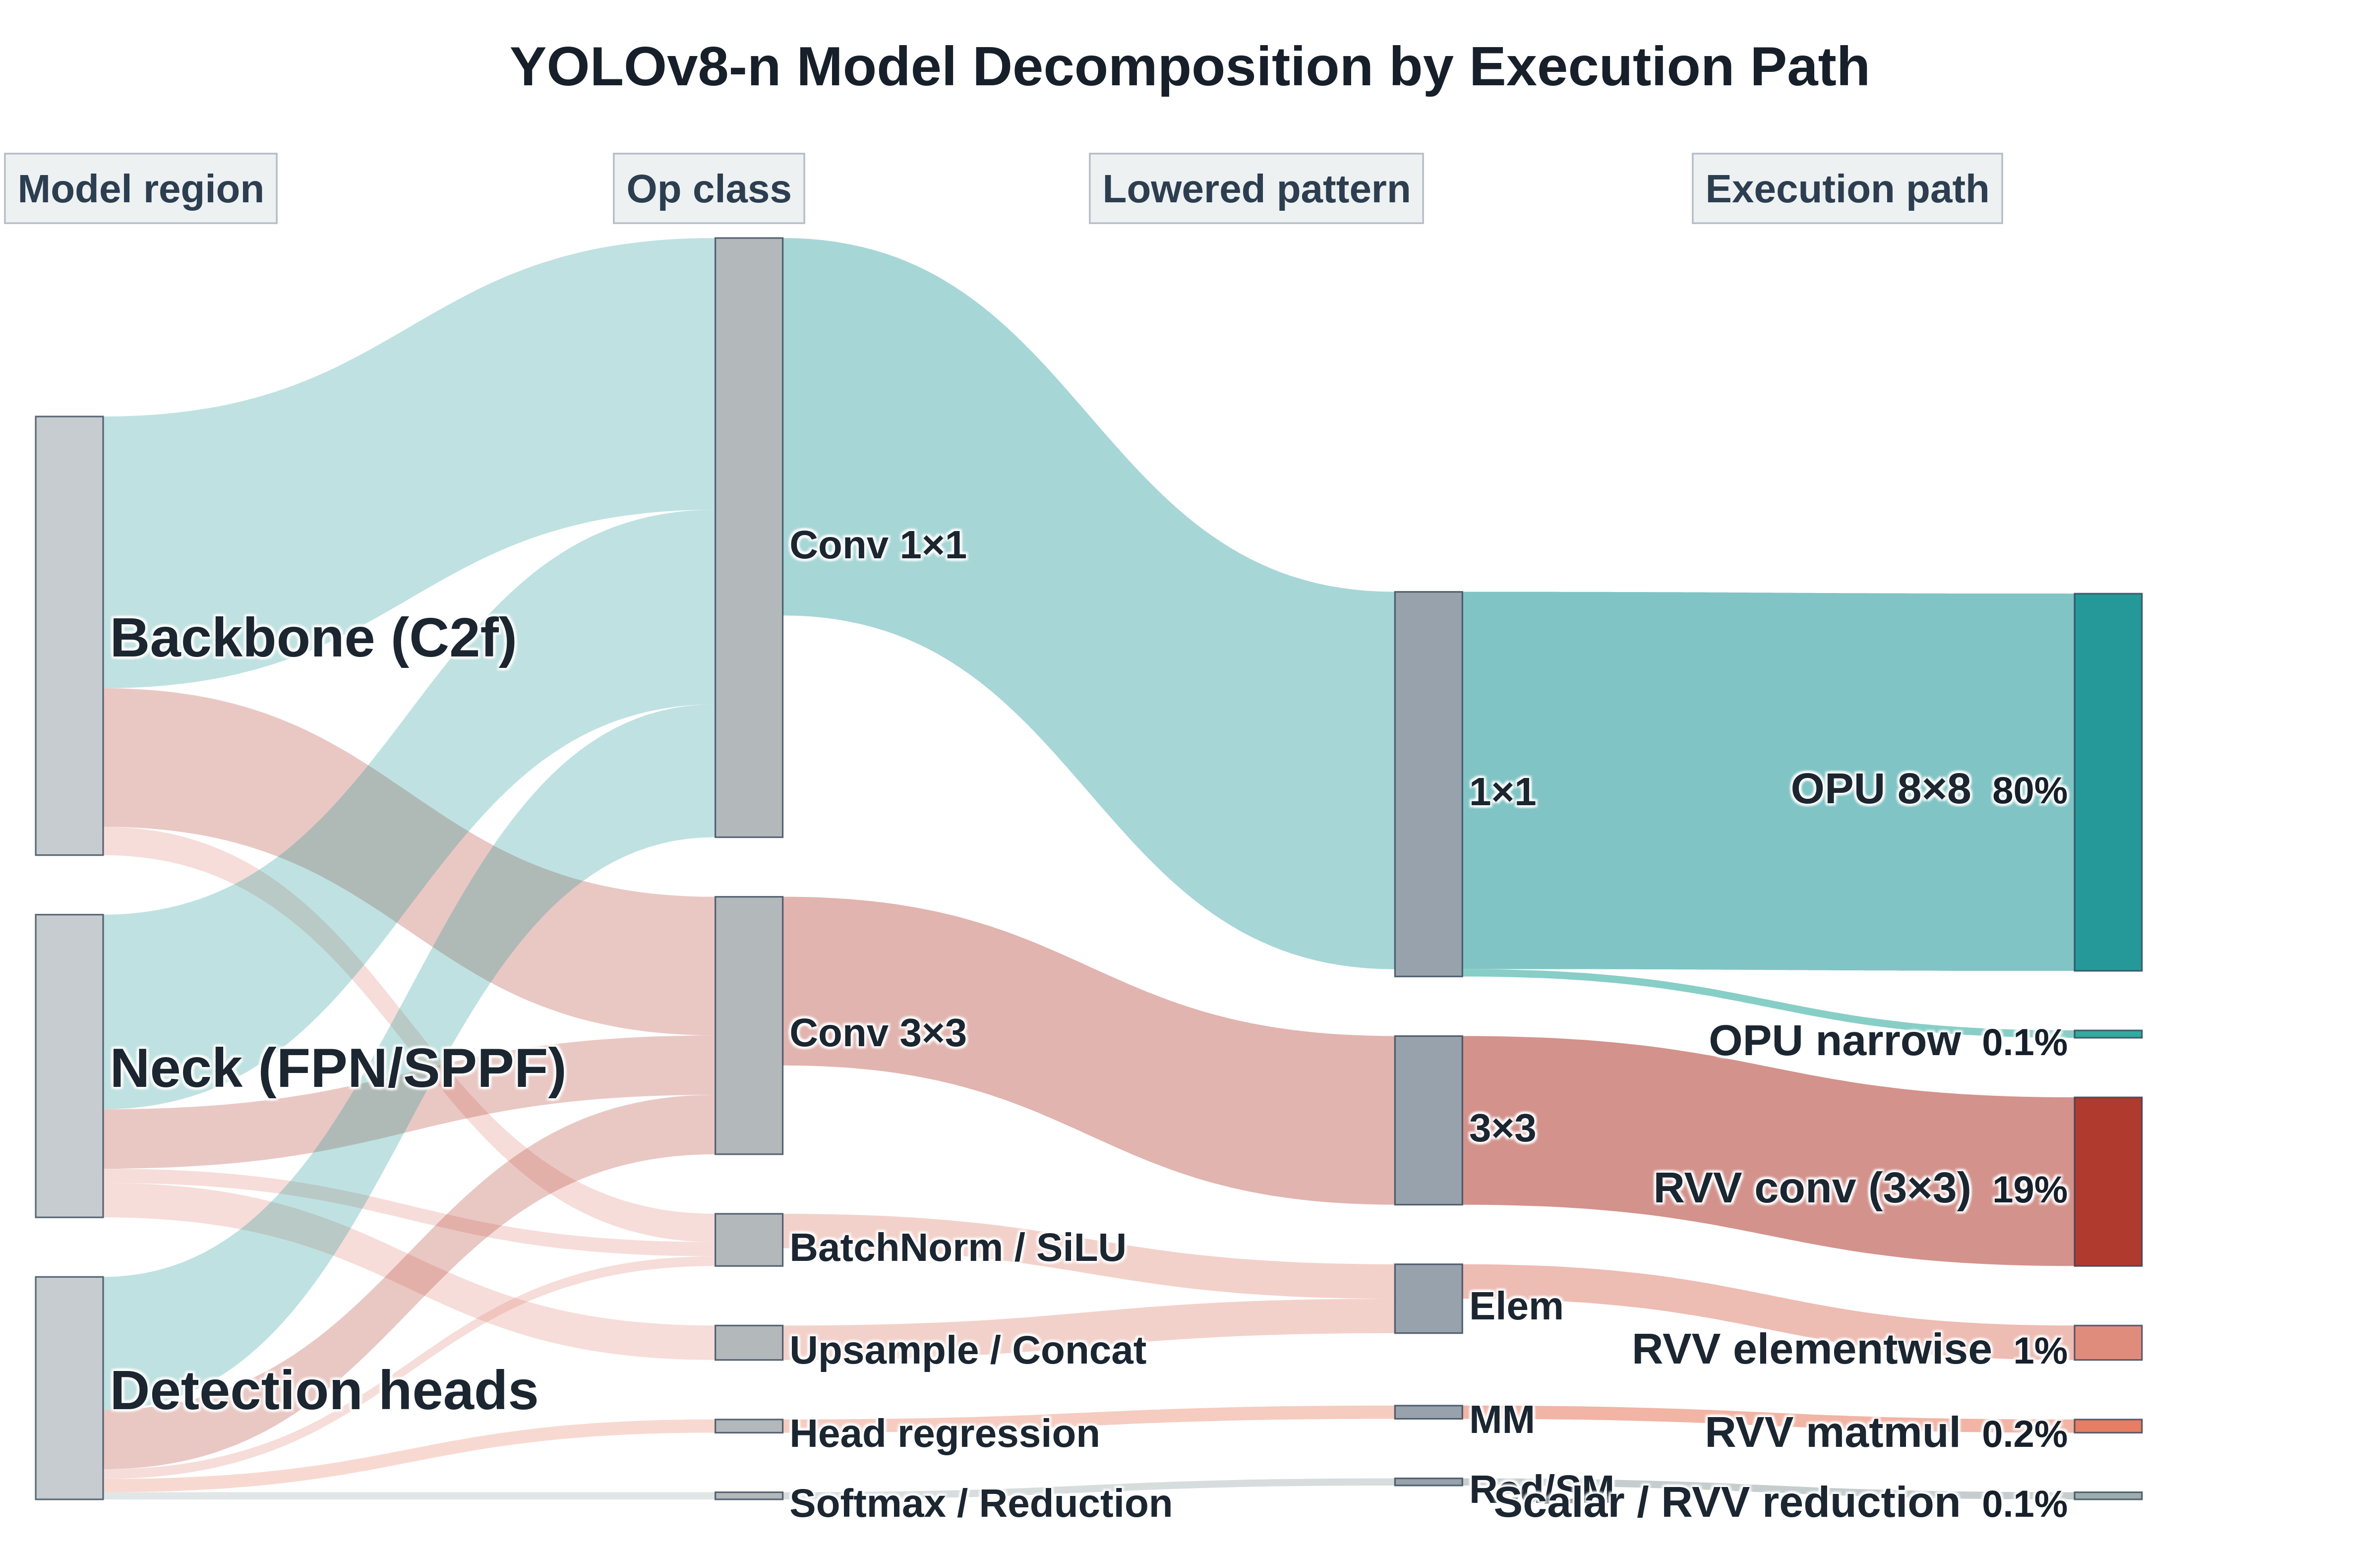
\includegraphics[width=\linewidth]{figures/sankey_yolov8_paper.png}
  \end{minipage}
  \caption{Two case studies showing how model regions are transformed into lowered compute patterns and final execution paths. Left: a hybrid CNN+transformer model, where attention projections, matmuls, and FFN layers lower primarily into OPU~32$\times$32 (77\% of analytical compute), while LayerNorm, softmax, and the convolution stem remain on scalar/RVV paths. Right: YOLOv8-n, where 1$\times$1 convolutions are converted via im2col into matmul and dispatched through the OPU~8$\times$8 runtime path (80\%), while 3$\times$3 convolutions remain as RVV spatial loops (19\%).}
  \label{fig:iree-sankey}
\end{figure*}

To make this transformation process explicit, Fig.~\ref{fig:iree-sankey} shows two representative models. Each diagram traces high-level model regions through intermediate lowered patterns to final execution families. The hybrid model (left) illustrates the transformer case: attention projections, FFN layers, and related dense subgraphs all converge into a shared batched-matmul lowering that maps to OPU~32$\times$32, while reductions, softmax, and direct convolution remain on non-OPU paths. YOLOv8-n (right) illustrates the CNN case: 1$\times$1 convolutions are rewritten through im2col into matmul and dispatched via the OPU~8$\times$8 runtime path, while 3$\times$3 spatial convolutions remain as RVV vector loops. In both cases, the compiler does not introduce one custom path per operator; instead, it reduces diverse layer families into a small set of contraction-oriented patterns that can share the same OPU lowering.

\begin{figure}[t]
  \centering
  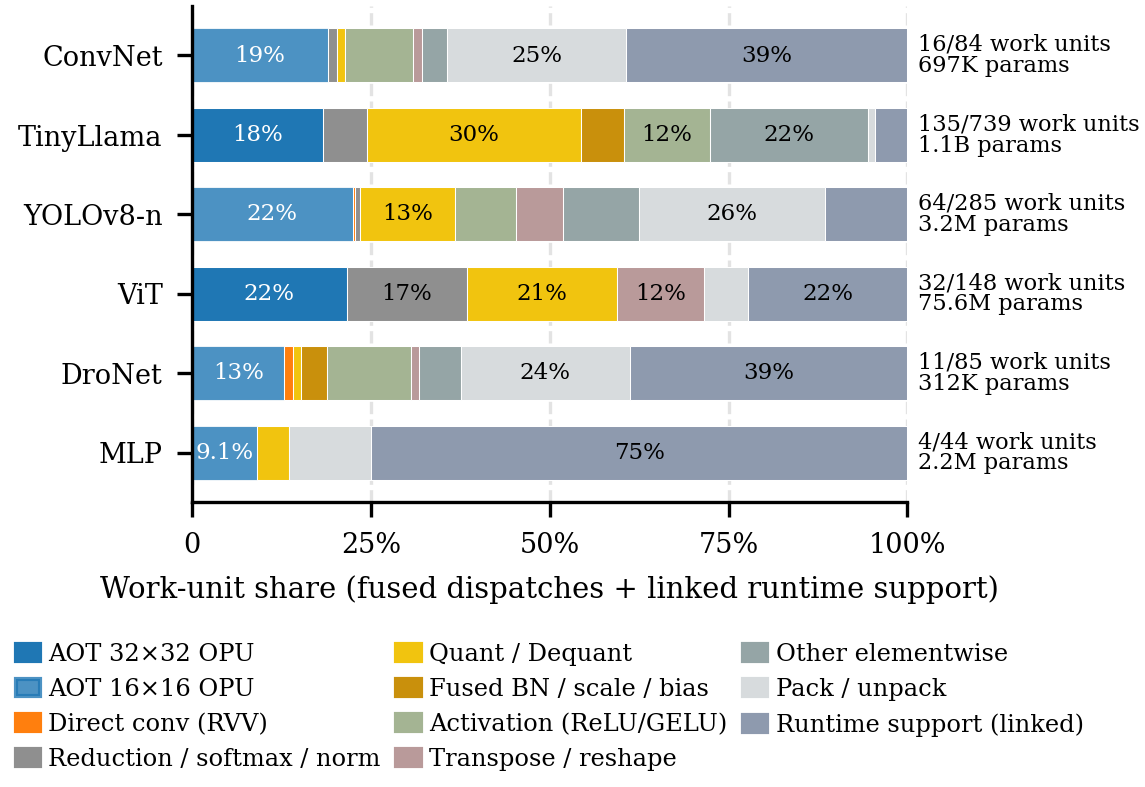
\includegraphics[width=\linewidth]{figures/per_model_decomposition_over110.png}
  \caption{Work-unit decomposition of compiled IREE artifacts across the validated end-to-end models. Each colored segment shows the fraction of work units assigned to one execution path. The annotation at right reports the percentage of work units that land on OPU-backed paths, the raw count (OPU work units / total work units), and the model's parameter count.}
  \label{fig:iree-model-decomposition}
\end{figure}

A \emph{work unit} is one fused block of computation the compiled binary invokes as a single call. It is the compiler's unit of scheduling, not a source-level operator: a \texttt{BatchNorm}, an activation, and a residual add often fuse into one work unit, while a quantized matmul typically expands into three (pre-pack, compute, requantize).

We extract work units with a small Python tool that reads the intermediate MLIR dumps and the linked RISC-V assembly, walks the function table, and keeps only the bodies the IREE front-end emitted. Linker-injected code---standard math helpers and the IREE runtime-query stub---is tallied separately as \emph{runtime support}. Each kept work unit is classified first from its body: if it contains the Saturn matrix outer-product instruction, the unit is OPU-backed, with the VOPACC count inside the inner loop deciding whether it is a 16$\times$16 or 32$\times$32 tile. Otherwise we read the compute kind and the I/O dtype suffix the compiler attached to the dispatch name. As a concrete example, a work unit whose signature reads \texttt{f32→i8} is a \emph{quantize} (input is float, output is int8), the reverse \texttt{i8→f32} is a \emph{dequantize}, and a body that takes an \texttt{i32} accumulator and writes \texttt{i8} is a \emph{requantize}; the same idea sorts activations (single dtype, no change), fused BatchNorm (three or more dtypes in the signature because the compiler chained scale, bias, and activation), and transpose/reshape (identity dtype, explicit layout change). The full rule table and the IR fragments we rely on are in the supplementary \emph{METHODS} appendix.

Figure~\ref{fig:iree-model-decomposition} shows the decomposition. Because work units vary by orders of magnitude in per-invocation cost, this view does not predict end-to-end speedup on its own. What the data shows instead is \emph{where the compiler's attention is}: a small cluster of OPU-backed kernels carrying the real work, and a much larger population of cheap glue operations around them---quantize, dequantize, requantize, pack/unpack, activations, and the linker-injected runtime helpers.

The three highest-speedup models---ConvNet (13.24$\times$), TinyLlama (10.97$\times$), and YOLOv8-n (10.38$\times$)---all have low OPU work-unit coverage (19.0\%, 18.3\%, 22.5\%), consistent with the view that the heavy kernels are few and the quant/activation/reshape glue is plentiful. What distinguishes them in the figure is the shape of the glue. TinyLlama spends most of its non-OPU work units on the quant/dequant/requant triad plus fused BN-style reductions, precisely the tax of running int8 attention at each layer boundary. ConvNet and YOLOv8-n spend proportionally more on pack/unpack because their convolutions go through the im2col-plus-matmul path. In all three cases the heavy OPU kernels dominate execution time even though they do not dominate the work-unit count. MLP-Wide is the cautionary case: 3 of its 43 work units are OPU-backed (7\%) but 77\% of the units are linker-injected runtime support, and the measured speedup is only 1.25$\times$. The model is too small for OPU to amortize the fixed cost of standing up the inference pipeline. Table~\ref{tab:iree-model-speedup-rvv} reports the realized end-to-end speedups.

\begin{table}[t]
  \centering
  \small
  \setlength{\tabcolsep}{6pt}
  \begin{tabular}{lc}
    \hline
    Model & Speedup over RVV \\
    \hline
    ConvNet   & 13.24$\times$ \\
    TinyLlama & 10.97$\times$ \\
    YOLOv8-n  & 10.38$\times$ \\
    DroNet    & 6.08$\times$ \\
    MLP-Wide  & 1.25$\times$ \\
    ViT       & 1.23$\times$ \\
    \hline
    Geomean   & 4.91$\times$ \\
    \hline
  \end{tabular}
  \caption{End-to-end speedup of the compiler-based Saturn IREE flow over the pure-RVV baseline for models with at least 1.10$\times$ speedup. Two additional models fall below this threshold: the Hybrid CNN+transformer model at 1.08$\times$ and a Large MLP at 0.52$\times$ (RVV is faster because the memory-bound \(K\!=\!512\) matmuls cannot saturate the OPU). Including all eight validated pairs yields a geomean of 3.07$\times$.}
  \label{tab:iree-model-speedup-rvv}
\end{table}

Taken together, the two software paths tell a consistent story. The library-based XNNPACK flow is the most useful environment for detailed kernel bring-up and measurement, and it exposes the layout, packing, and dispatch effects that dominate kernel-level performance. The compiler-based IREE flow lifts those same lessons to the graph level by rewriting more of the model into OPU-supported kernel families, which increases model coverage and yields substantial end-to-end gains even after accounting for the surrounding system overheads.
